% LaTeX Template for short student reports.
% Citations should be in bibtex format and go in references.bib
\documentclass[a4paper, 11pt]{article}
\usepackage[top=3cm, bottom=3cm, left = 2cm, right = 2cm]{geometry} 
\geometry{a4paper} 
\usepackage[utf8]{inputenc}
\usepackage{textcomp}
\usepackage{graphicx} 
\usepackage{amsmath,amssymb}  
\usepackage{bm}  
\usepackage{float}
\usepackage[pdftex,bookmarks,colorlinks,breaklinks]{hyperref}  
\hypersetup{linkcolor=black,citecolor=black,filecolor=black,urlcolor=black} % black links, for printed output
\usepackage{float}
\usepackage{memhfixc} 
\usepackage{pdfsync}  
\usepackage{xcolor}
\usepackage{booktabs}
\usepackage{tikz}
\usetikzlibrary{positioning, calc}

\title{Overview of calc3}
\author{Hossein Afkar}
%\date{}

\begin{document}
\maketitle
% \tableofcontents

\section{Calc3 design description}
\subsection{Overview of the system}
In this section we describe the Calc3 system in which we are tasked with the
verification of its design. Calc3 is an ALU calculator that has 16 registers
for keeping the internal state. Because of this change, arithmetic operands are
no longer sent by the requestor instead we have the fetch and store commands
which will change the state of the registers according to the commands we
issue. Also in addition to the fetch and store commands, we have two new branch
commands which will cause the next command from the port to be skipped. Each
requestor can send up to 4 commands concurrently with a 2 bit tag on request.
Using the same tag on consequent commands is not supported. In this design we
have operand and source registers therefore, instruction ordering must be 
obeyed in order to keep the machine state clean and correct and also to
avoid data and control hazards. There are four sets of inputs and outputs
with "X" denoted in the port tags Figure~\ref{figure:1}.

\begin{figure}[H]
    \centering
    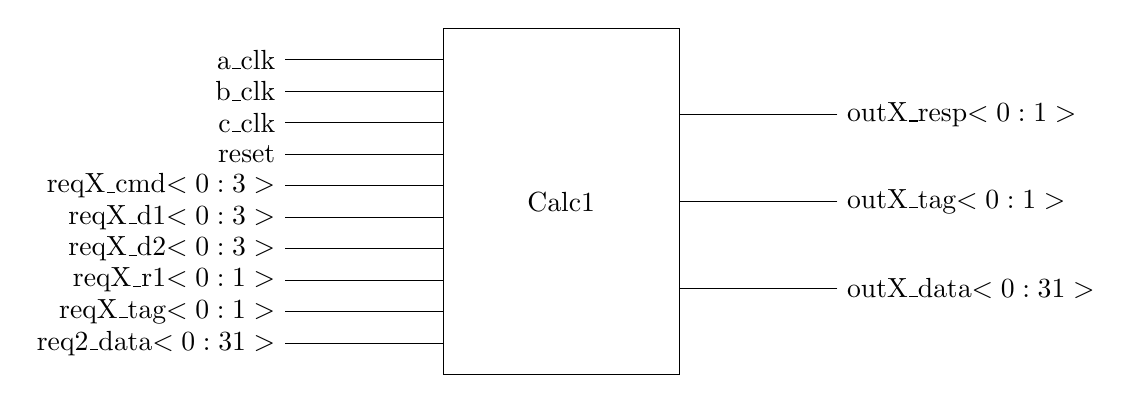
\begin{tikzpicture}
        \node (rectangle) [draw, rectangle, minimum width = 3 cm, minimum
        height = 4.4 cm] (Y) at (4,0) {Calc1} ;
        \draw [-] ($(Y.west) + (0,1.8)$) -- ++ (-2, 0) node [pos = 1, left]
        {a\_clk};
        \draw [-] ($(Y.west) + (0,1.4)$) -- ++ (-2, 0) node [pos = 1, left]
        {b\_clk};
        \draw [-] ($(Y.west) + (0,1.0)$) -- ++ (-2, 0) node [pos = 1, left]
        {c\_clk};
        \draw [-] ($(Y.west) + (0,0.6)$) -- ++ (-2, 0) node [pos = 1, left]
        {reset};
        \draw [-] ($(Y.west) + (0,0.2)$) -- ++ (-2, 0) node [pos = 1, left]
        {reqX\_cmd$<0:3>$};
        \draw [-] ($(Y.west) + (0,-0.2)$) -- ++ (-2, 0) node [pos = 1, left]
        {reqX\_d1$<0:3>$};
        \draw [-] ($(Y.west) + (0,-0.6)$) -- ++ (-2, 0) node [pos = 1, left]
        {reqX\_d2$<0:3>$};
        \draw [-] ($(Y.west) + (0,-1.0)$) -- ++ (-2, 0) node [pos = 1, left]
        {reqX\_r1$<0:1>$};
        \draw [-] ($(Y.west) + (0,-1.4)$) -- ++ (-2, 0) node [pos = 1, left]
        {reqX\_tag$<0:1>$};
        \draw [-] ($(Y.west) + (0,-1.8)$) -- ++ (-2, 0) node [pos = 1, left]
        {req2\_data$<0:31>$};
        \draw [-] ($(Y.east) + (2,1.1)$) -- ++ (-2, 0) node [pos = 0, right]
        {outX\_resp$<0:1>$};
        \draw [-] ($(Y.east) + (2,0)$) -- ++ (-2, 0) node [pos = 0, right]
        {outX\_tag$<0:1>$};
        \draw [-] ($(Y.east) + (2,-1.1)$) -- ++ (-2, 0) node [pos = 0, right]
        {outX\_data$<0:31>$};
    \end{tikzpicture}
    \caption{Calc3 inputs and outputs diagram}
    \label{figure:1}
\end{figure}
\pagebreak
\noindent Calc3 command decode values are shown in Table~\ref{table:1}.
\begin{table}[H]
    \centering
    \begin{tabular}{ll}
        \toprule
        Command & Decode value \\
        \cmidrule(r){1-1}\cmidrule(lr){2-2}
        No operation & "0000"b\\
        Add & "0001"b\\
        Subtract & "0010"b\\
        Shift left & "0101"b\\
        Shift right& "0110"b\\
        Store& "1001"b\\
        Fetch& "1010"b\\
        Branch if zero& "1100"b\\
        Branch if equal& "1101"b\\
        Invalid & All others\\
        \bottomrule
    \end{tabular}
    \caption{Calc3 command decode values}
    \label{table:1}
\end{table}
Calc3 response values that are put on out\_Xresp port are shown in
Table~\ref{table:2}.
\begin{table}[H]
    \centering
    \begin{tabular}{lp{12cm}l}
        \toprule
        Response decode & Response meaning\\
        \cmidrule(r){1-1}\cmidrule(lr){2-2}
        "01"b & Successful operation.\\
        "10"b & Overflow/underflow error.\\
        "11"b & Command skipped due to branch.\\
        \bottomrule
    \end{tabular}
    \caption{Calc3 command output values}
    \label{table:2}
\end{table}
Calc3 has three additional commands in compared to Calc3. Because of the
transition to the ALU style design we have fetch, store, and branch commands
available in the design. Also it is stated in the design sheet that we should
leave a dead cycle between commands. There are rules within each port
instruction stream that consists of some logic that prevents data hazards.
In short no consecutive commands can write while the prior commands has
RAW or WAR hazards. But this will not prevent this kinds of hazards in other
ports instruction stream.
Verification plan for Calc3 is based on the blackbox method. In 
Figure~\ref{figure:3} we have a simple diagram for the basic verification
environment. The stimulus and responder get data from the input ports and
the checker and monitor share the output ports and collect all the data.
The scoreboard monitors the checker and stimulus responder and collects the
result for further checking.

\begin{figure}[H]
    \centering


\tikzset{every picture/.style={line width=0.75pt}} %set default line width to 0.75pt        

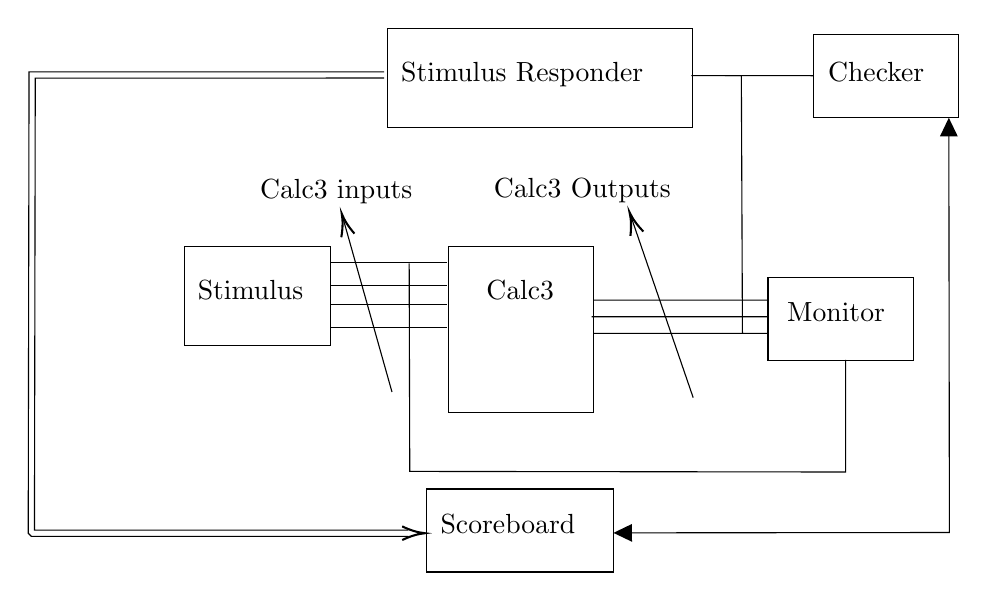
\begin{tikzpicture}[x=0.75pt,y=0.75pt,yscale=-1,xscale=1]
%uncomment if require: \path (0,300); %set diagram left start at 0, and has height of 300

%Shape: Rectangle [id:dp5697228224002759] 
\draw   (289,122) -- (359,122) -- (359,202.03) -- (289,202.03) -- cycle ;
%Straight Lines [id:da7189033070332109] 
\draw    (232.47,130.03) -- (288.47,130.03) ;
%Straight Lines [id:da3679326207032825] 
\draw    (232.47,150.03) -- (288.47,150.03) ;
%Straight Lines [id:da2467980653011279] 
\draw    (232.47,161.03) -- (288.47,161.03) ;
%Straight Lines [id:da40577994176378085] 
\draw    (232.47,141.03) -- (288.47,141.03) ;
%Shape: Rectangle [id:dp38730159512477735] 
\draw   (162,122) -- (232,122) -- (232,170.03) -- (162,170.03) -- cycle ;
%Straight Lines [id:da36353370229719206] 
\draw    (261.83,192.24) -- (238.16,108.24) ;
\draw [shift={(237.62,106.31)}, rotate = 74.26] [color={rgb, 255:red, 0; green, 0; blue, 0 }  ][line width=0.75]    (10.93,-3.29) .. controls (6.95,-1.4) and (3.31,-0.3) .. (0,0) .. controls (3.31,0.3) and (6.95,1.4) .. (10.93,3.29)   ;
%Shape: Rectangle [id:dp00024023325823807617] 
\draw   (259.47,17) -- (406.47,17) -- (406.47,65.03) -- (259.47,65.03) -- cycle ;
%Straight Lines [id:da0035156306852393016] 
\draw    (258,41) -- (89.97,41.03) -- (89.58,258.8) -- (269.68,258.8)(258,38) -- (86.97,38.03) -- (86.58,260.29) -- (88.08,261.8) -- (269.68,261.8) ;
\draw [shift={(277.68,260.3)}, rotate = 180] [color={rgb, 255:red, 0; green, 0; blue, 0 }  ][line width=0.75]    (10.93,-3.29) .. controls (6.95,-1.4) and (3.31,-0.3) .. (0,0) .. controls (3.31,0.3) and (6.95,1.4) .. (10.93,3.29)   ;
%Shape: Rectangle [id:dp16545893981577753] 
\draw   (278.47,239) -- (368.47,239) -- (368.47,279) -- (278.47,279) -- cycle ;
%Shape: Rectangle [id:dp07836664435212337] 
\draw   (443,137) -- (513,137) -- (513,177) -- (443,177) -- cycle ;
%Shape: Rectangle [id:dp6076948567540941] 
\draw   (464.71,20) -- (534.71,20) -- (534.71,60) -- (464.71,60) -- cycle ;
%Straight Lines [id:da34666593411430635] 
\draw    (359,148) -- (443.47,148.03) ;
%Straight Lines [id:da07946846692295706] 
\draw    (359,164) -- (443.47,164.03) ;
%Straight Lines [id:da8652457234478481] 
\draw    (358,156) -- (443.47,156.03) ;
%Straight Lines [id:da2510318754395182] 
\draw    (406.08,39.85) -- (430.16,39.85) -- (430.69,164.16) ;
%Straight Lines [id:da2590031738964804] 
\draw    (422.16,39.85) -- (464.69,39.87) ;
%Straight Lines [id:da1385589744718032] 
\draw    (270.12,130.24) -- (270.4,230.52) -- (480.4,230.81) -- (480.4,176.81) ;
%Straight Lines [id:da4874312895005559] 
\draw    (530.12,63.16) -- (530.4,259.96) -- (371.54,260.13) ;
\draw [shift={(368.54,260.14)}, rotate = 359.94] [fill={rgb, 255:red, 0; green, 0; blue, 0 }  ][line width=0.08]  [draw opacity=0] (8.93,-4.29) -- (0,0) -- (8.93,4.29) -- cycle    ;
\draw [shift={(530.12,60.16)}, rotate = 89.92] [fill={rgb, 255:red, 0; green, 0; blue, 0 }  ][line width=0.08]  [draw opacity=0] (8.93,-4.29) -- (0,0) -- (8.93,4.29) -- cycle    ;
%Straight Lines [id:da6207609853062772] 
\draw    (406.95,194.98) -- (376.93,107.54) ;
\draw [shift={(376.28,105.64)}, rotate = 71.05] [color={rgb, 255:red, 0; green, 0; blue, 0 }  ][line width=0.75]    (10.93,-3.29) .. controls (6.95,-1.4) and (3.31,-0.3) .. (0,0) .. controls (3.31,0.3) and (6.95,1.4) .. (10.93,3.29)   ;

% Text Node
\draw (167,137) node [anchor=north west][inner sep=0.75pt]   [align=left] {Stimulus};
% Text Node
\draw (197,88.67) node [anchor=north west][inner sep=0.75pt]   [align=left] {Calc3 inputs};
% Text Node
\draw (306,137) node [anchor=north west][inner sep=0.75pt]   [align=left] {Calc3};
% Text Node
\draw (265,32) node [anchor=north west][inner sep=0.75pt]   [align=left] {Stimulus Responder};
% Text Node
\draw (284,250) node [anchor=north west][inner sep=0.75pt]   [align=left] {Scoreboard};
% Text Node
\draw (451,148) node [anchor=north west][inner sep=0.75pt]   [align=left] {Monitor};
% Text Node
\draw (470.71,32) node [anchor=north west][inner sep=0.75pt]   [align=left] {Checker};
% Text Node
\draw (309.67,88) node [anchor=north west][inner sep=0.75pt]   [align=left] {Calc3 Outputs};


\end{tikzpicture}
    \caption{Calc3 verification environment}
    \label{figure:3}
\end{figure}

\subsection{Verification scenarios}
Here we have some verification scenarios which are based on the examples of the
book. \\
\begin{table}[H]
    \centering
    \begin{tabular}{lp{12cm}l}
        \toprule
        Test refrence number& Test description\\
        \cmidrule(r){1-1}\cmidrule(lr){2-2}
        1.1 & Check the basic command response of the four ports. \\
        1.2 & Check the basic operation of each command on each port.\\
        1.3 & Check the overflow and underflow cases for add and subtracts \\
        1.4 & Check if the reset functionality correctly resets the design\\
        \bottomrule
    \end{tabular}
    \caption{Calc3 basic functionality test}
    \label{table:3}
\end{table}

\begin{table}[H]
    \centering
    \begin{tabular}{lp{12cm}l}
        \toprule
        Test refrence number& Test description\\
        \cmidrule(r){1-1}\cmidrule(lr){2-2}
        2.1 & For each port and register combination check that the add, subtract,
        and shift results are correct\\
        2.1.1 & Data dependent corner case: Check the overflow and 
        underflow situations \\
        2.1.2 & Data dependent corner case: Check shift 0 and 31 places 
        with all register combinations \\
        2.2 & For each port and register combination check that each command
        can follow any other add or subtract command without 
        leaving the design dirty\\
        2.3 & Check that for each port can access all the registers with any
        commands \\
        2.4 & Check that the design correctly handles bnez on all registers \\
        2.5 & Check that the design correctly handles bez on all registers \\
        2.6 & On each port check that for any combination of commands
        the branch correctly skips one command \\
        2.7 & On each port check for RAW hazards on the same ports \\
        2.8 & On different ports check for RAW hazards on the same ports \\
        2.9 & On each port check for WAR hazards on the same ports \\
        2.10 & On different ports check for WAR hazards on the same ports \\
        2.11 & Check that for each port we can store to any register \\
        2.12 & Check that for each port we can load from any register \\
        2.13 & Check that for each port we can have any combination of loads
        and stores following a command that operated on the same register\\
        2.14 & Corner Case: Check that one shift and add command from different
        ports can access same registers \\
        2.15 & Corner Case: Issue a branch after filling every port with
        add commands \\
        2.16 & Corner Case: Issue four branches on each port with the same
        destination and registers\\
        2.17 & Corner Case: On each port issue commands with all the
        available tags \\
        \bottomrule
    \end{tabular}
    \caption{Calc3 adder, branch, shift, and store functionality test}
    \label{table:4}
\end{table}

\begin{table}[H]
    \centering
    \begin{tabular}{lp{12cm}l}
        \toprule
        Test refrence number& Test description\\
        \cmidrule(r){1-1}\cmidrule(lr){2-2}
        3.1 & On each port issue a command with same source and output
        registers at same time \\
        3.1.1 & On each port check that all add/sub commands can follow each
        other with the same registers \\
        3.2 & On each port check that issuing four branch operations 
        simultaneously on the same register correctly skips four 
        consecuent commands \\
        3.3 & Corner Case: Issue branch and change the condition on 
        different ports \\
        3.4 & Corner Case: For each port fill the priority buffer with any 
        commands and check that we can have another command follow it \\
        \bottomrule
    \end{tabular}
    \caption{Calc3 priority stage functionality test}
    \label{table:5}
\end{table}

\end{document}
